\documentclass{beamer}
\usepackage{preamble}
\usepackage{beamerPreamble}
\title{
    \Large \scshape \bf Don't Shit where You Drill!
}

\author{
    Michel Hardenberg\\ \tiny
    PhD student at AU - Quantifying the Vadose Zone\\
    Department of Electrical and Computer Engineering}

\date{
    \tiny
    \scshape 
    \centering
    \vspace{1em}
    
\includegraphics[width=0.25\textwidth]{mslogo} \\ 
Climate Justice Society
\today
}


\includeonly{
}

\begin{document}
\fontfamily{lmr}\selectfont

\begin{frame}
    \center{
        \Huge \scshape \bf Don't Shit where You Drill!
    }
    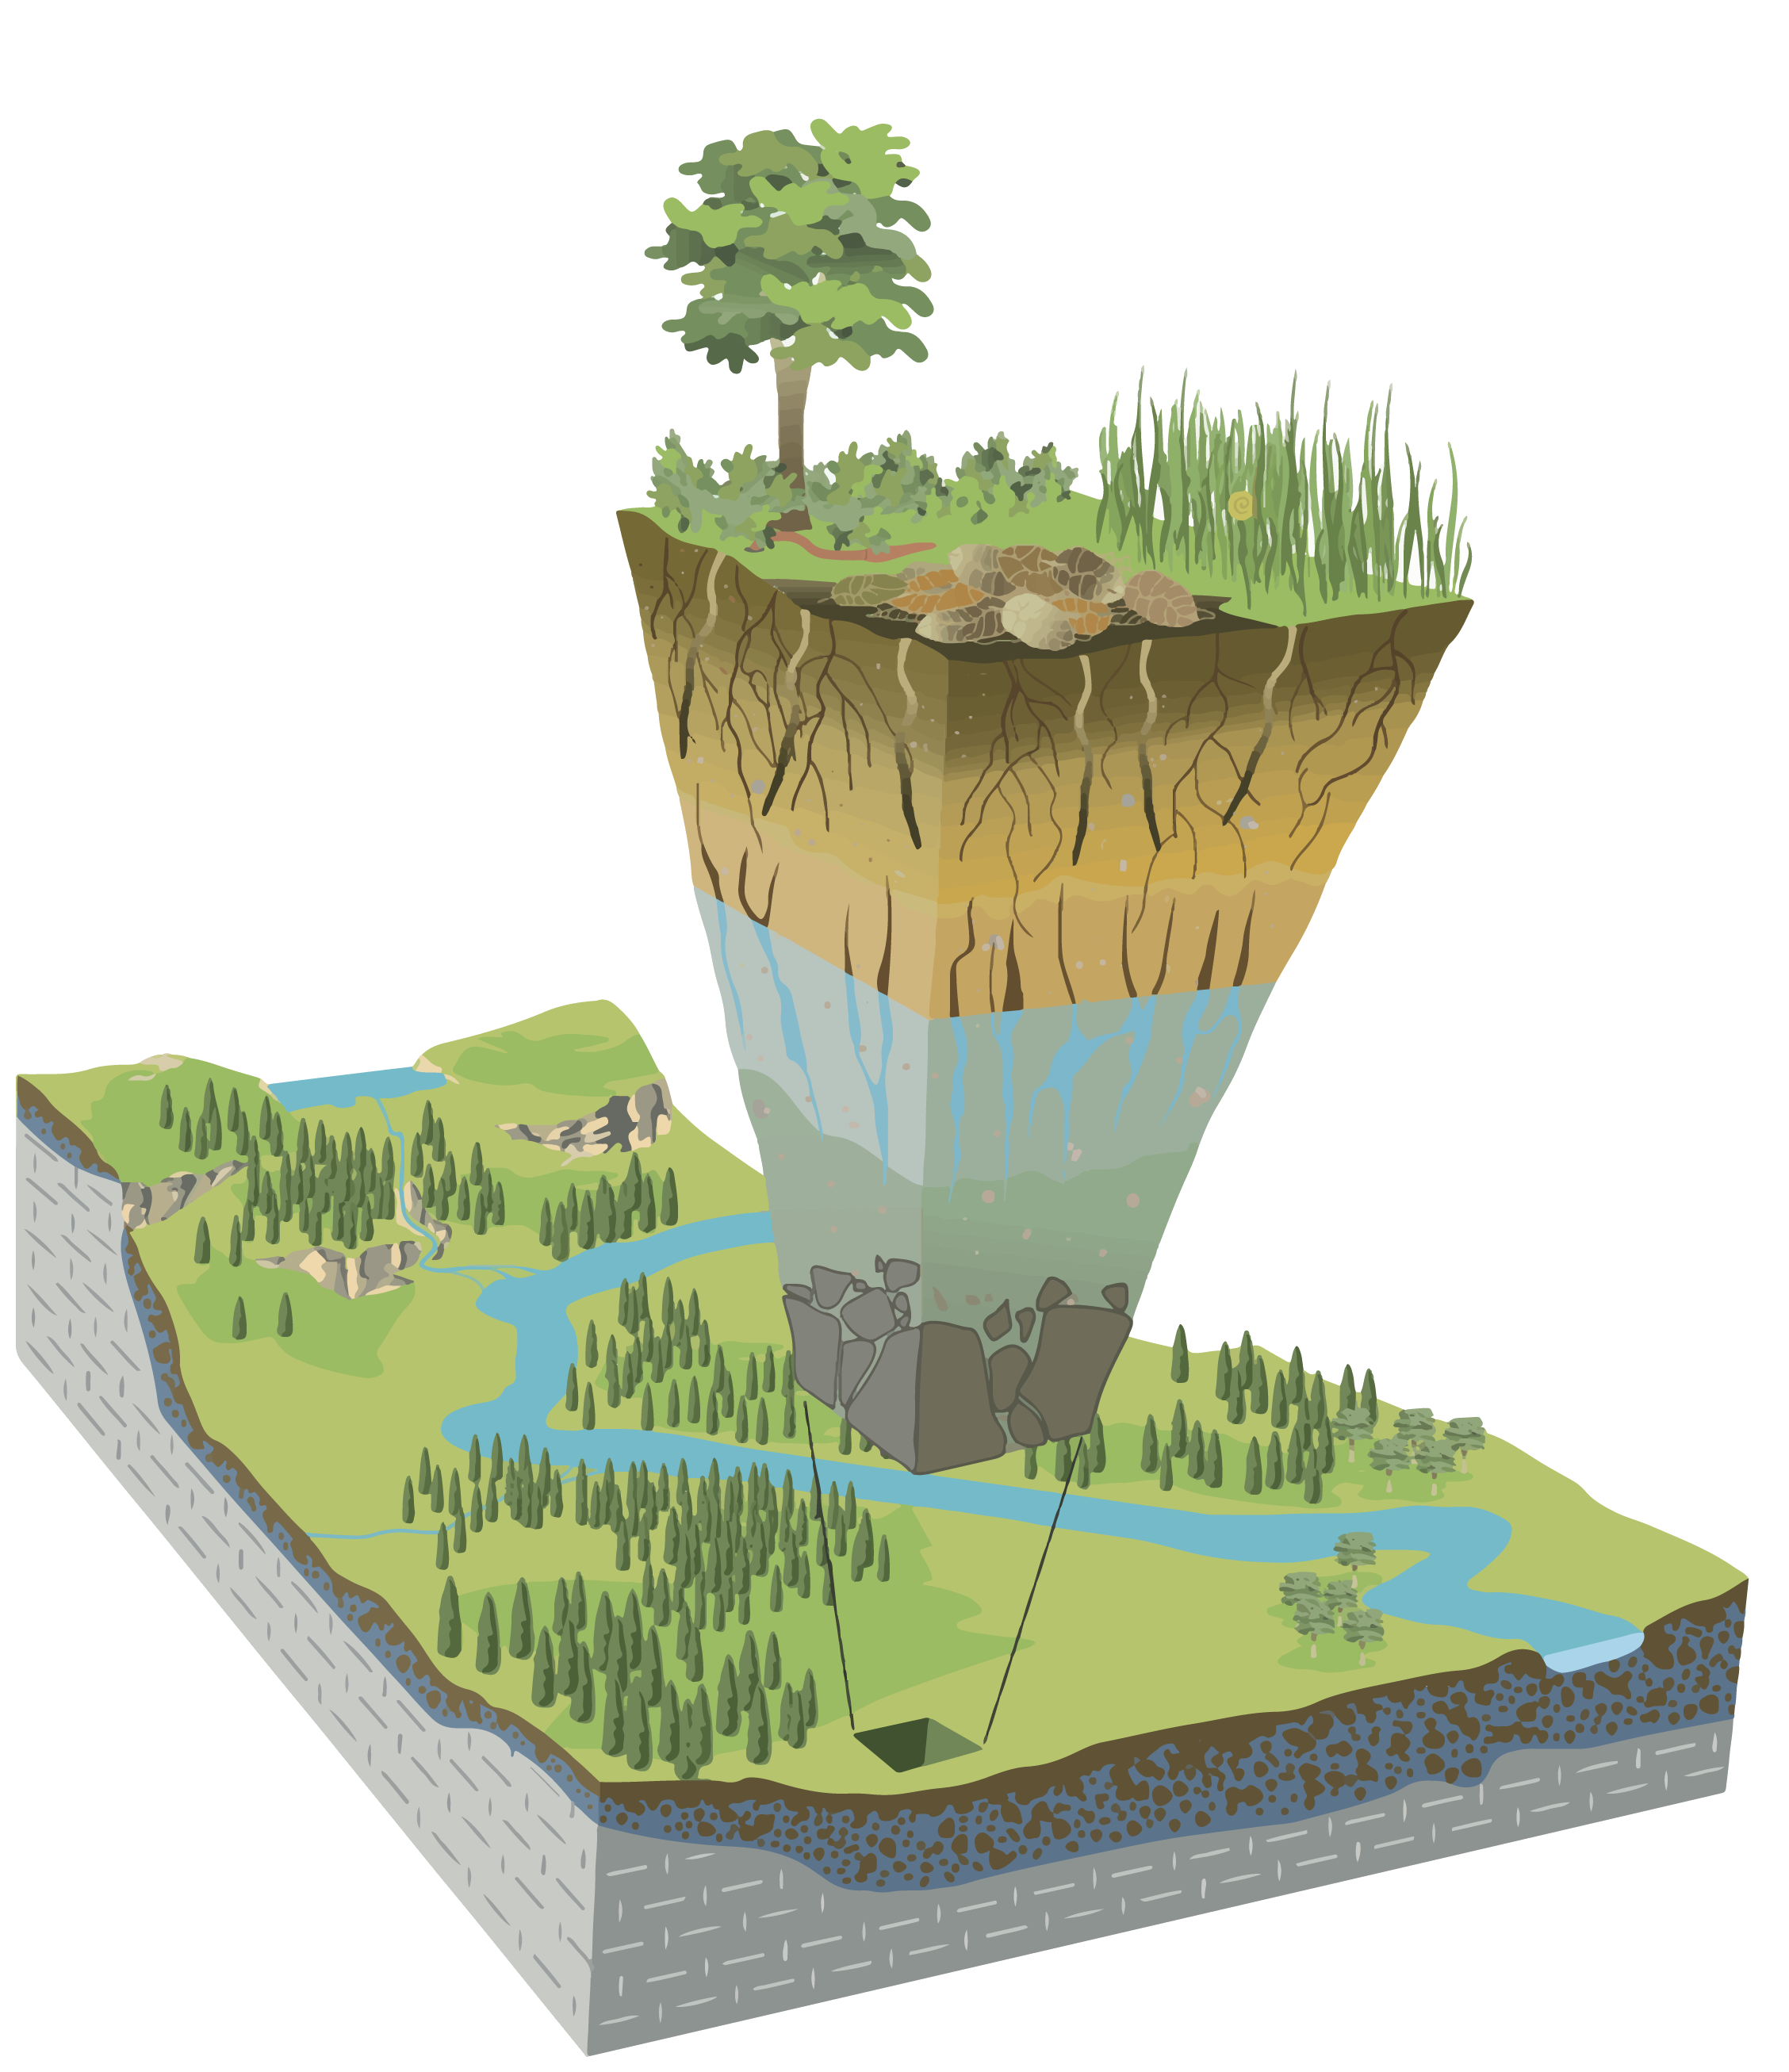
\includegraphics[width=1\textwidth]{figures/CriticalZoneStripped}

\end{frame}

\frame{\titlepage}

\begin{frame}
    \begin{minipage}{.9\columnwidth}
        \centering
        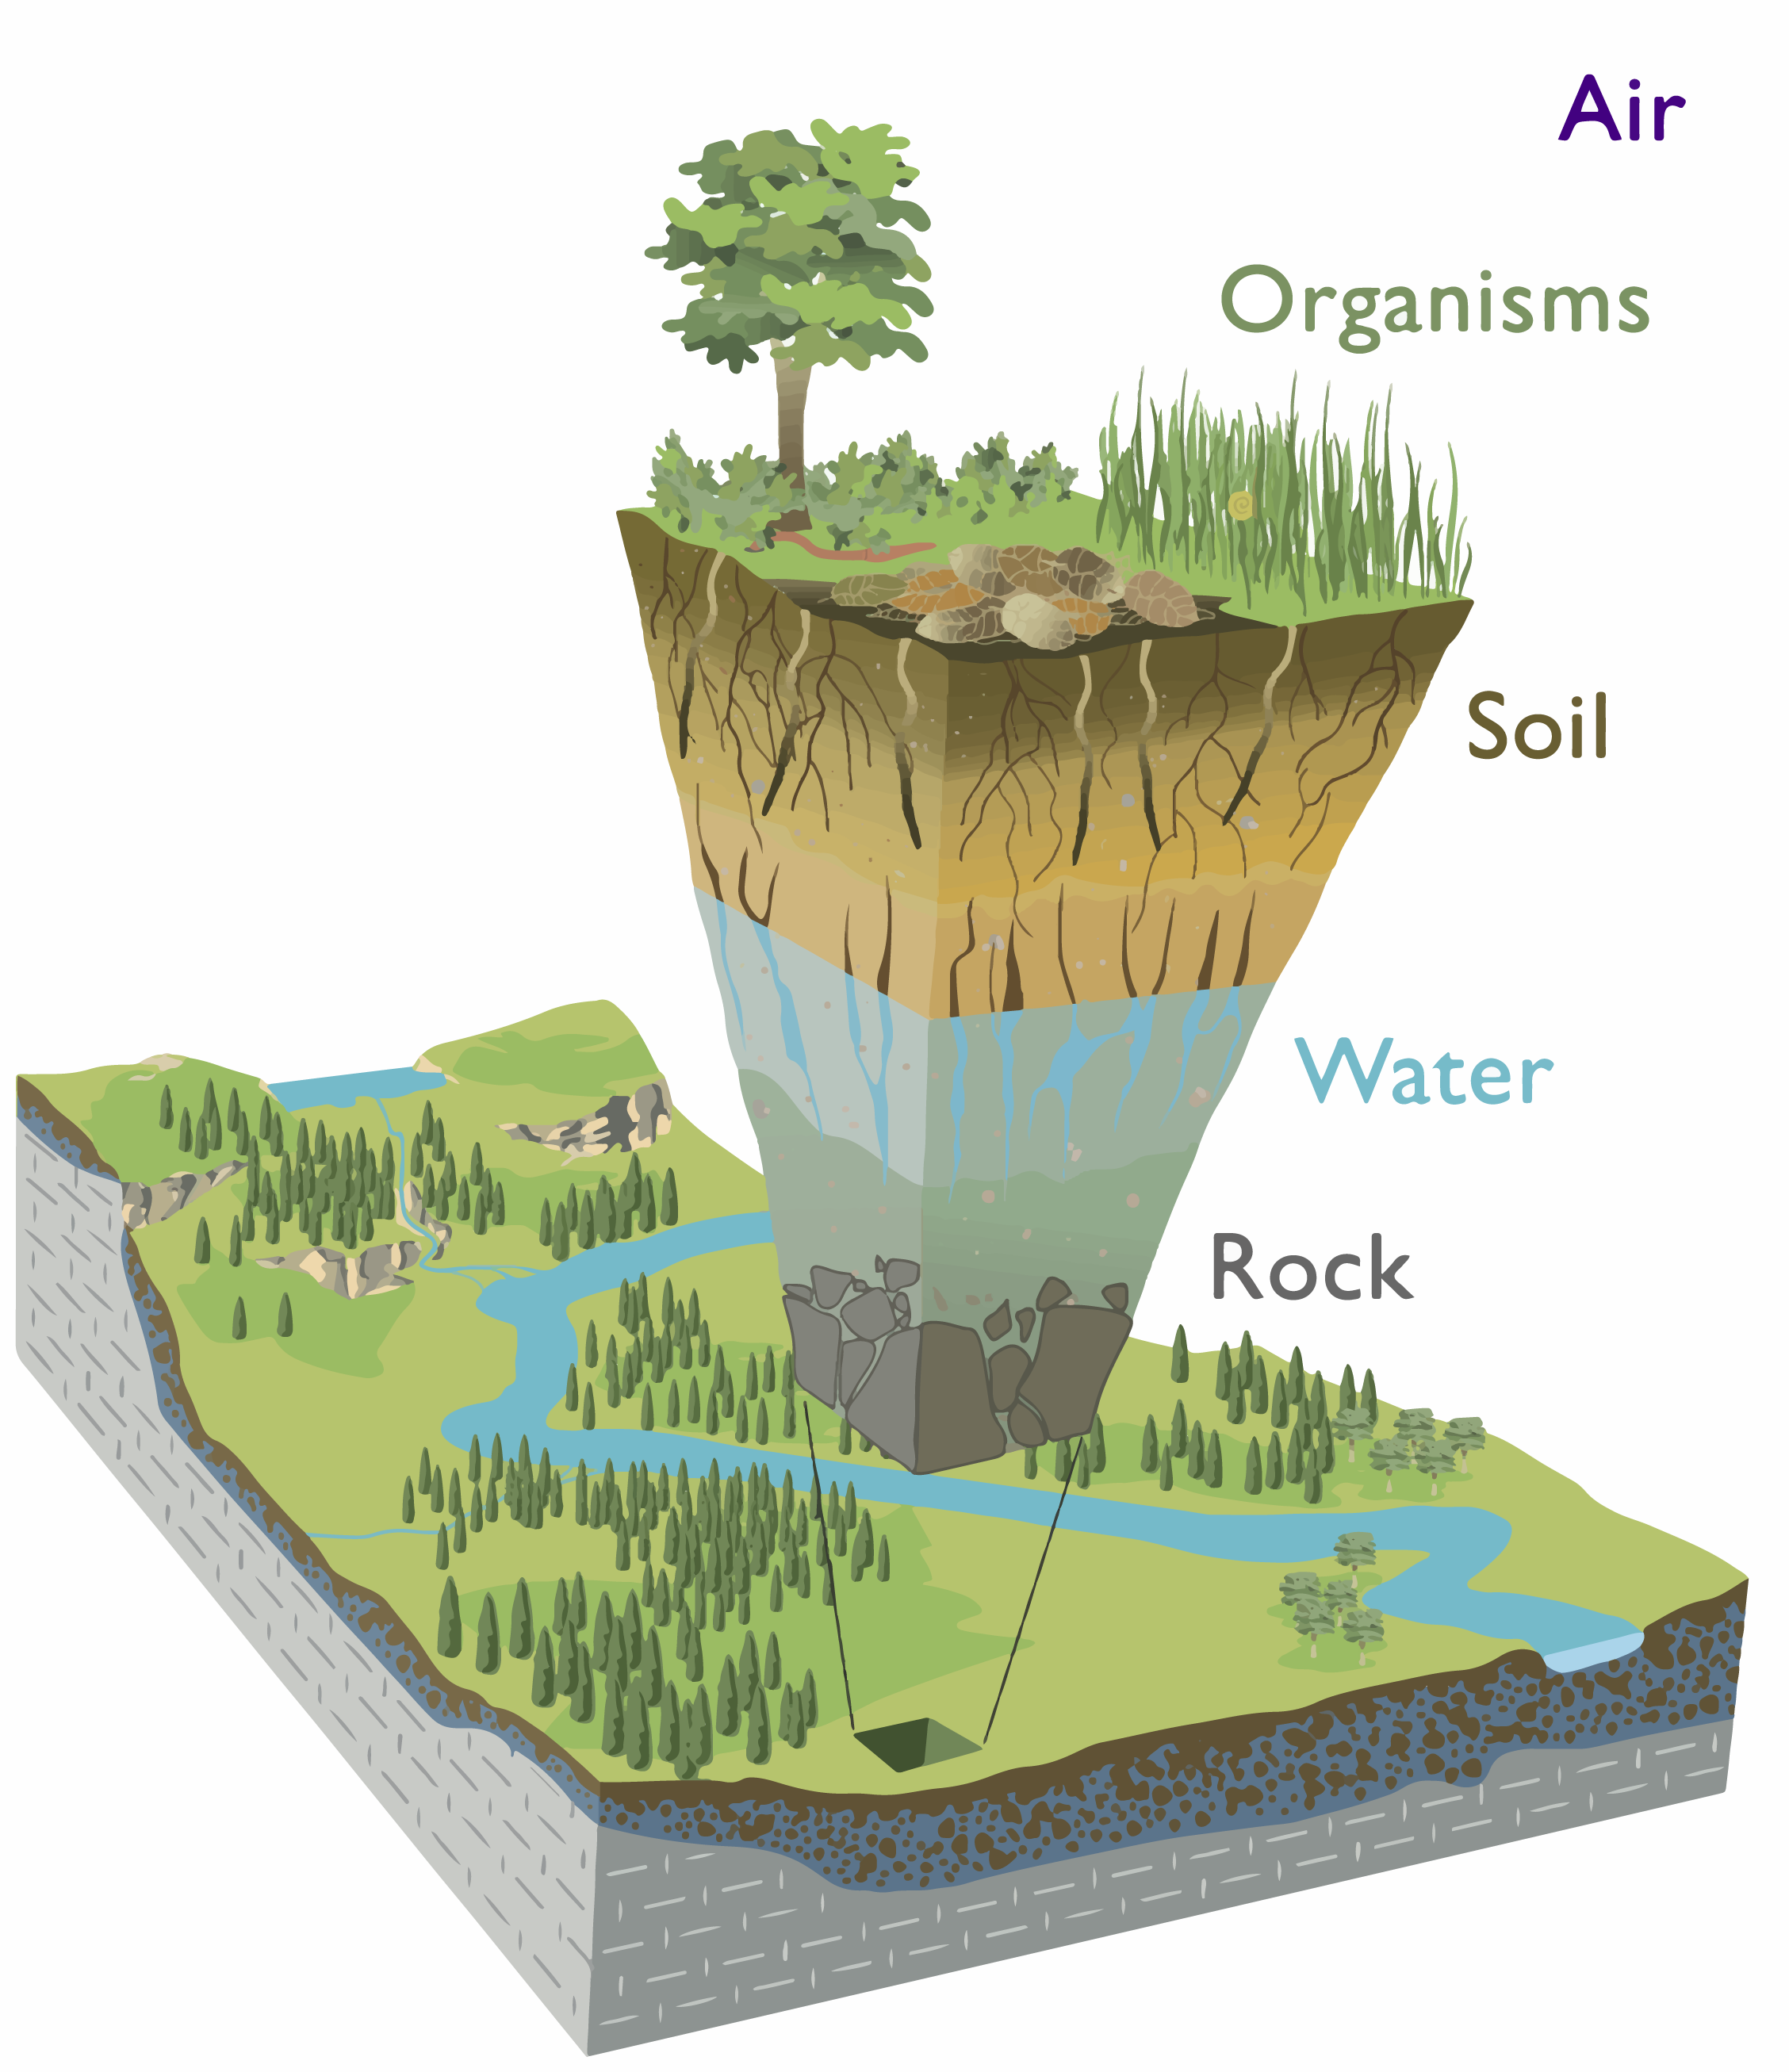
\includegraphics[width=.5\textwidth]{figures/CriticalZone.png}
        \vspace{8pt}
        \captionof{figure}{\it \footnotesize Illustration of soil layers
        in the near surface~\cite{chorover_soil_2007}.}
        \vspace{1em}
    \end{minipage}
\end{frame}

% Part 1
% -----------------------------------------------------------------------------
\begin{frame}{ToC}
    \begin{multicols}{2}
   \Large{Part One:}
    \begin{itemize}
        \item What are the culprits?
        \item How are we looking?
        \item What is the government doing? Promising?
    \end{itemize}\columnbreak


        \begin{minipage}{.5\textwidth}
            \center
        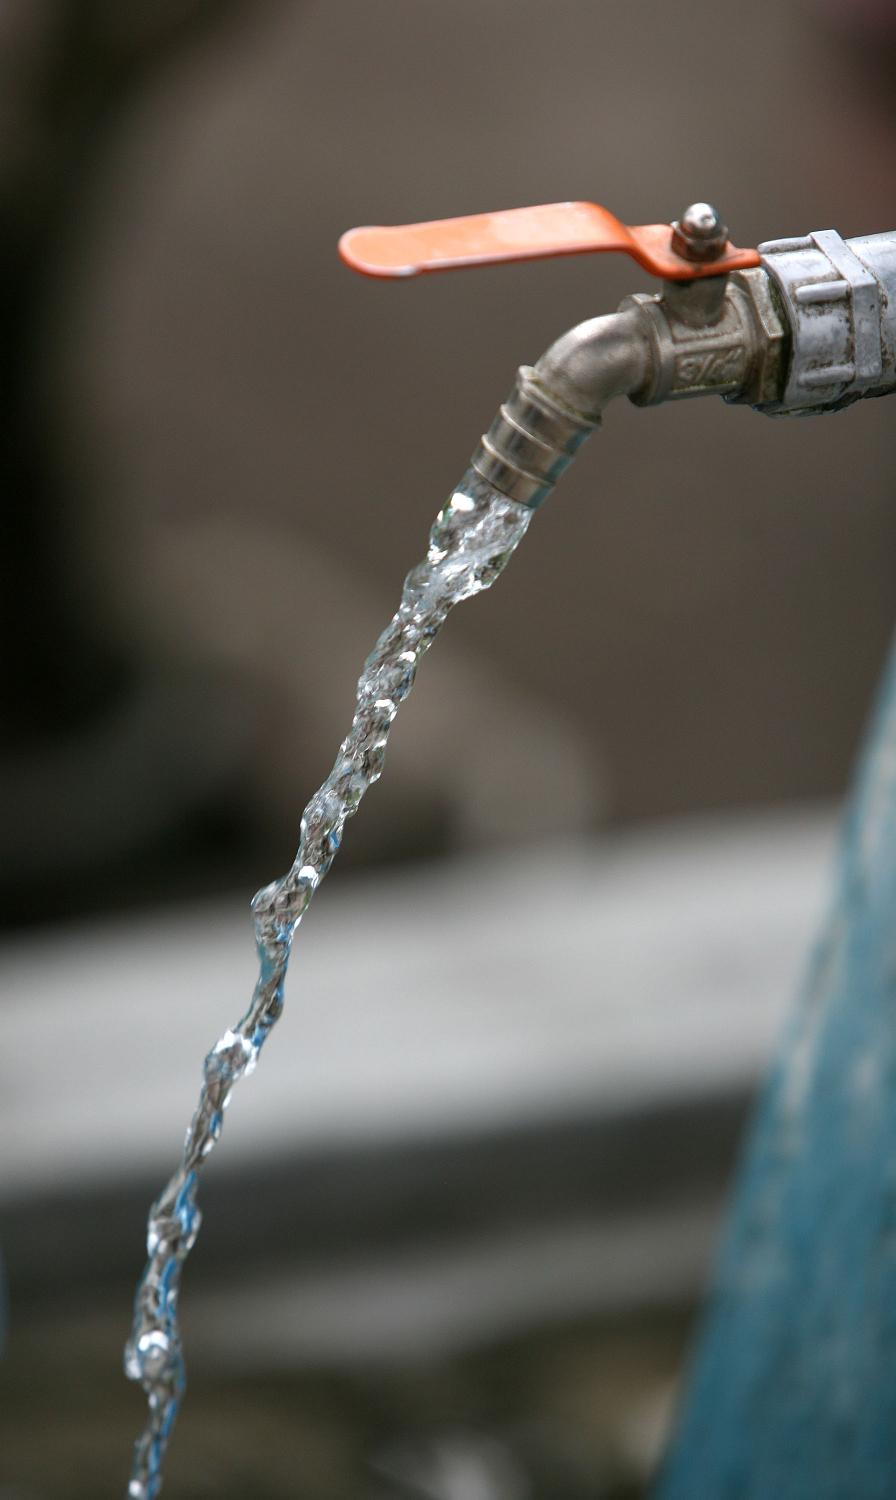
\includegraphics[width=.8\textwidth]{figures/tap.jpg}
        \end{minipage}
    \end{multicols}
\end{frame}

\begin{frame}{Denmark's water}
    \center
    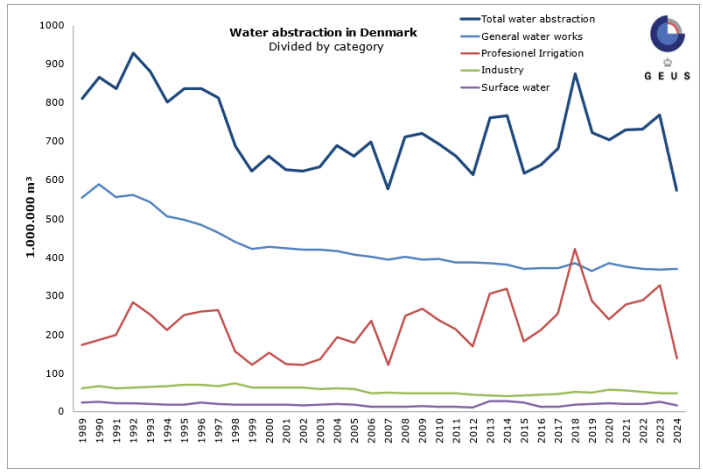
\includegraphics[width=.85\textwidth]{figures/waterAbstraction.png}
    \captionof{figure}{ \footnotesize From GEUS' groundwater report
    2025~\cite{laerke_thorling_groundwater_2025}.}
\end{frame}

\begin{frame}{GEUS water eport 2025}
    \begin{multicols}{2}
        \begin{description}\footnotesize
            \item<2->[Pesticides] are found in 70\% of testcites. 1 out of 3 exceeds the safety limits.
            \item<3->[Nitrate] from excessive farming reaches high concentrations in 1 out of 3 sites.
                16\% break the limits. In shallow depth sites 31\% do.
            \item<4>[PFAS] can be measured in every third site.
                The four highly regulated compounds\footnote[frame]{PFOS, PFOA, PFBS, PFHxS} in
                24\%.
        \end{description}
        \columnbreak

        \begin{minipage}{.45\textwidth}
            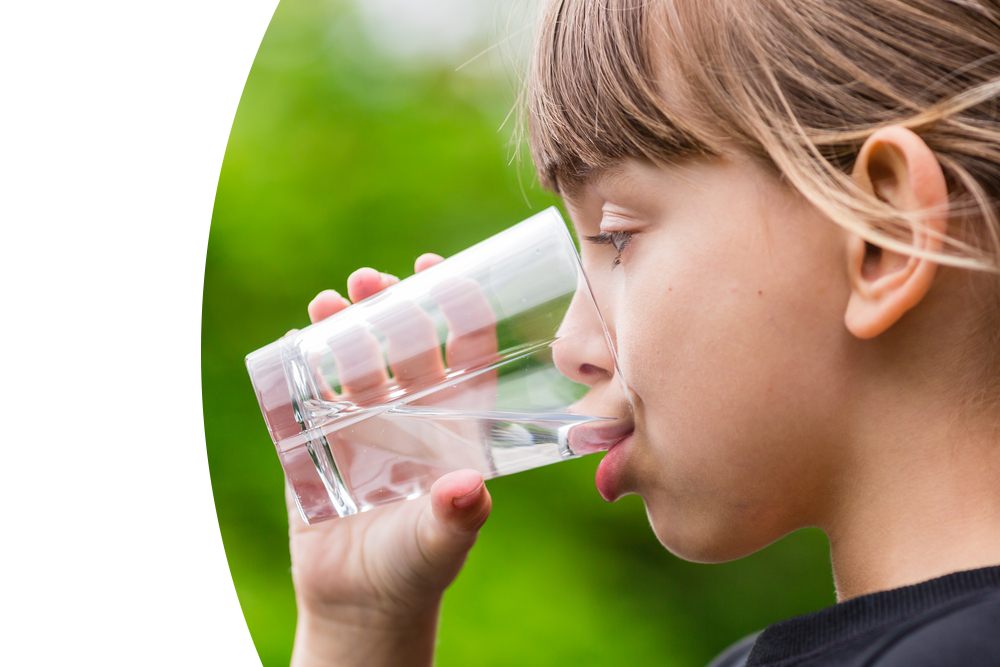
\includegraphics[height=1\textwidth]{figures/drinking.png}
        \end{minipage}

    \end{multicols}
\end{frame}

\begin{frame}
        \begin{center}
            \center
        
\includegraphics[width=\textwidth]{figures/wrestlingNO3.png}
        \end{center}

    \Huge\bf
    \textcolor{msred}{
    Nitrate - the Classic}


\end{frame}


\begin{frame}
    \center 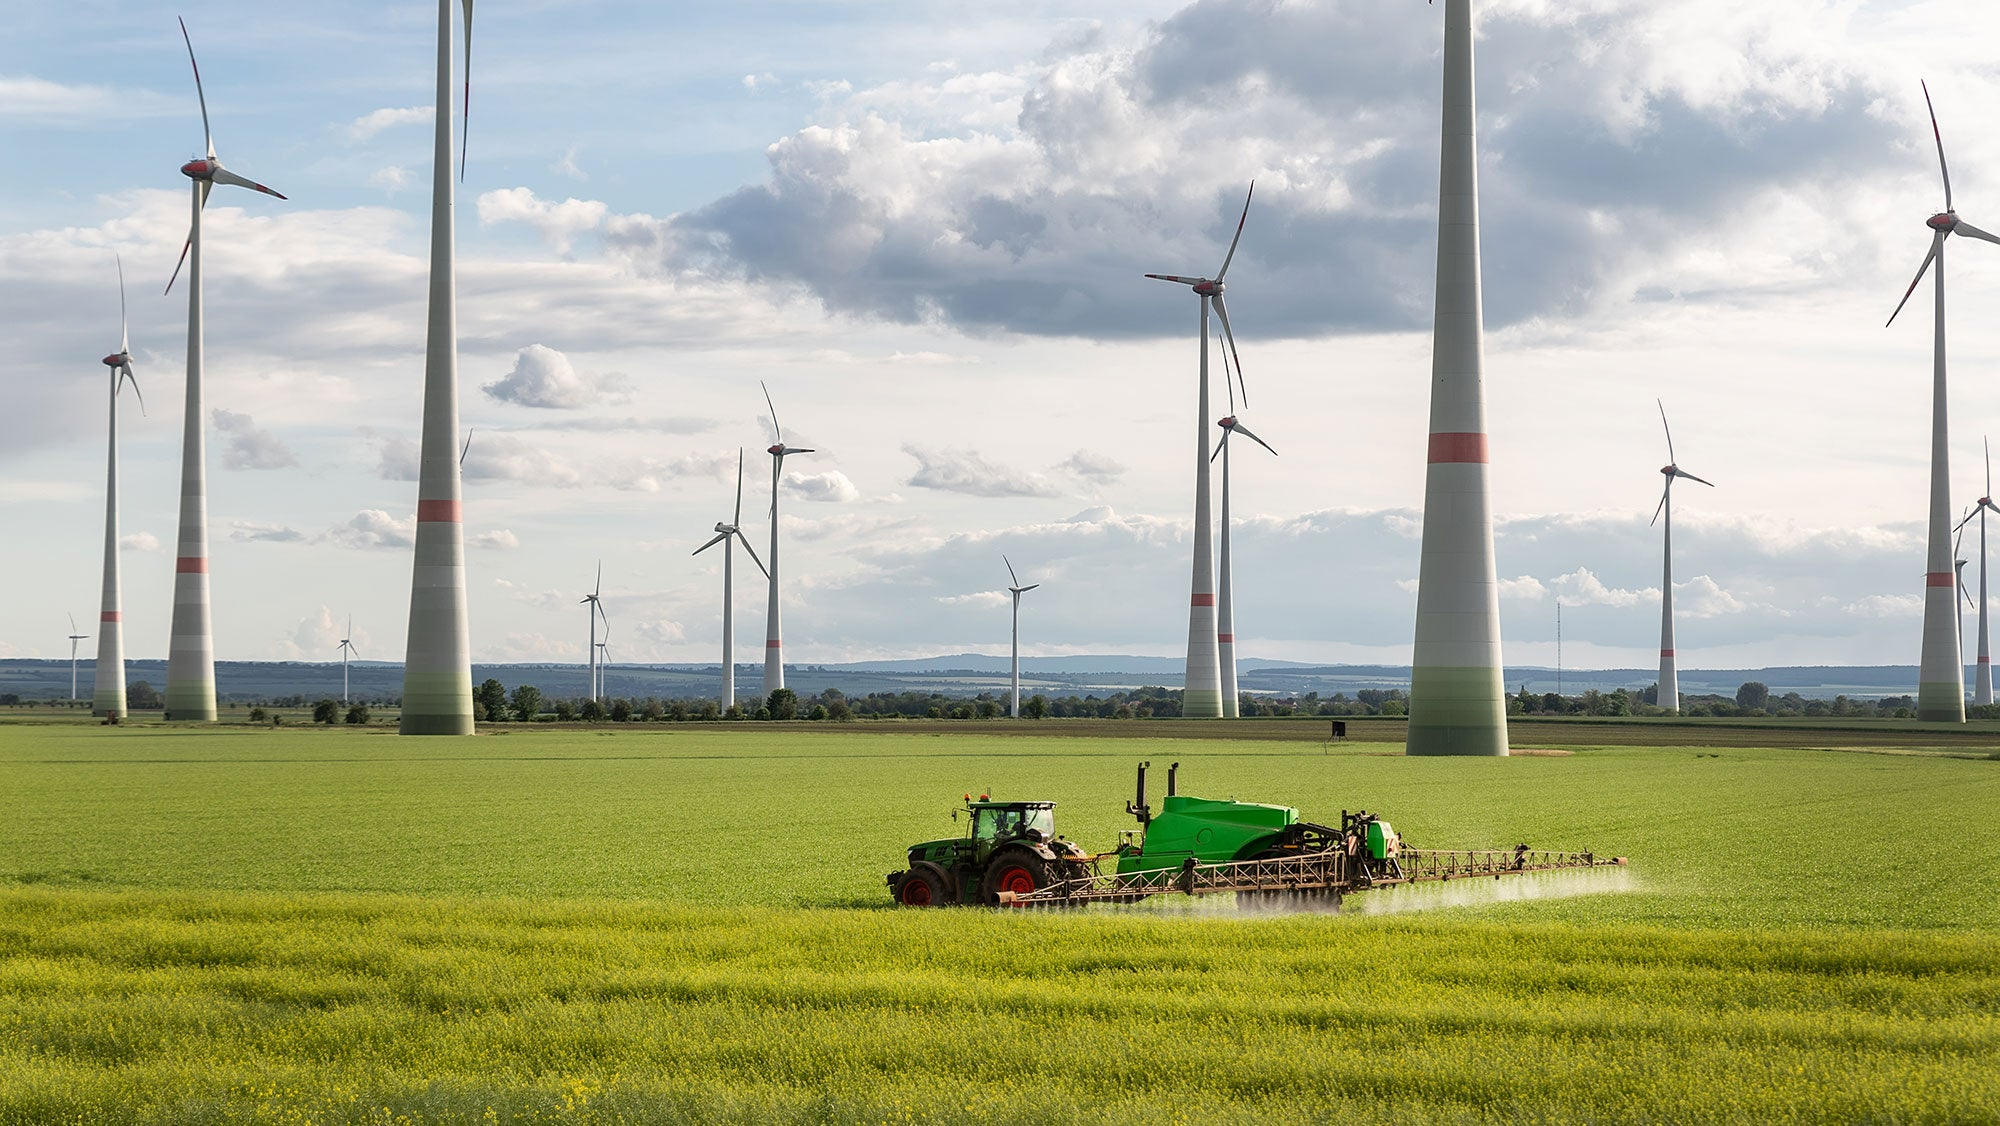
\includegraphics[width = .8\textwidth]{figures/farming.jpg}
\end{frame}

\begin{frame}
    \center 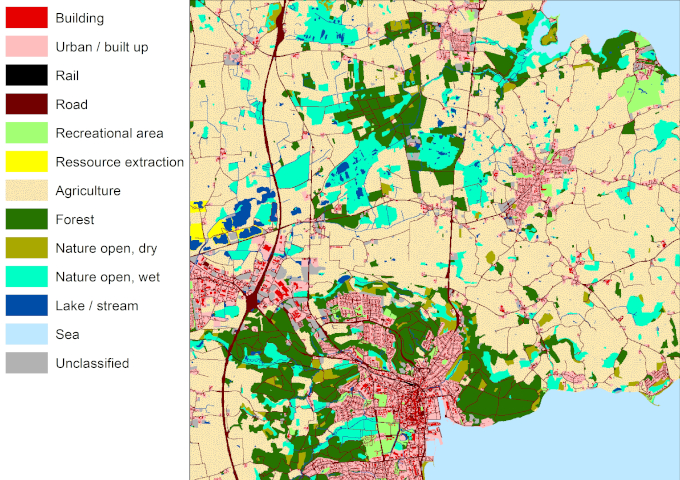
\includegraphics[width = .8\textwidth]{figures/farmland.jpg}
    More than half of the area of Denmark is used for agriculture!\footnote[frame]{\url{https://www.dst.dk/en/Statistik/emner/miljoe-og-energi/areal/arealopgoerelser}}
\end{frame}

\begin{frame}{Consequences}
    \begin{description}
        \item[Environmental]
            Pollution of bodies of water. Excess algae
            growth, extinction of fauna etc.
    \end{description}
\end{frame}

\begin{frame}{Consequences from the tab}

    \emph{
        “Nitrate in drinking water is a contaminant which can affect
        human health and has been associated with an increased risk
        of, amongst other diseases, colorectal
    cancer".}~\cite{jacobsen_health-economic_2024}\vspace{1em}

    \emph{
        For over 60 years, the global guideline for nitrates in drinking
        water has been 50 milligrams per litre (mg/L) [...] set in
        the 1950s\footnote[frame]{
    \url{https://www.greenpeace.org/international/story/82511/industrial-agriculture-profits-toxic-nitrates-pollution-tap-water/}}.}
\end{frame}

\begin{frame}
    \textcolor{msred}{\large This limit is hopelessly out of date}\vspace{1em}

    Literature proposes lower limits of $<10\%$ reducing the risk by $15\%$.
    Even lower limits of $<4\%$ bring this number down
    further~\cite{jacobsen_health-economic_2024, schullehner_nitrate_2018}.

\end{frame}

\begin{frame}{Nitrate pollution in Denmark}
    \center 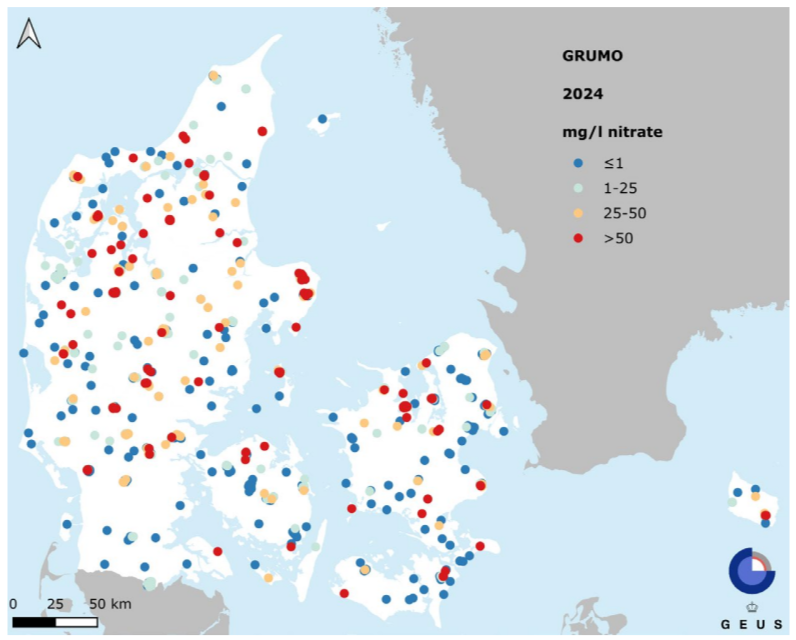
\includegraphics[width = .8\textwidth]{figures/grumoMapNitrate.png}
    \captionof{figure}{ \footnotesize From GEUS' groundwater report
    2025~\cite{laerke_thorling_groundwater_2025}.}
\end{frame}

\begin{frame}{Mixing and exploting}
    \center 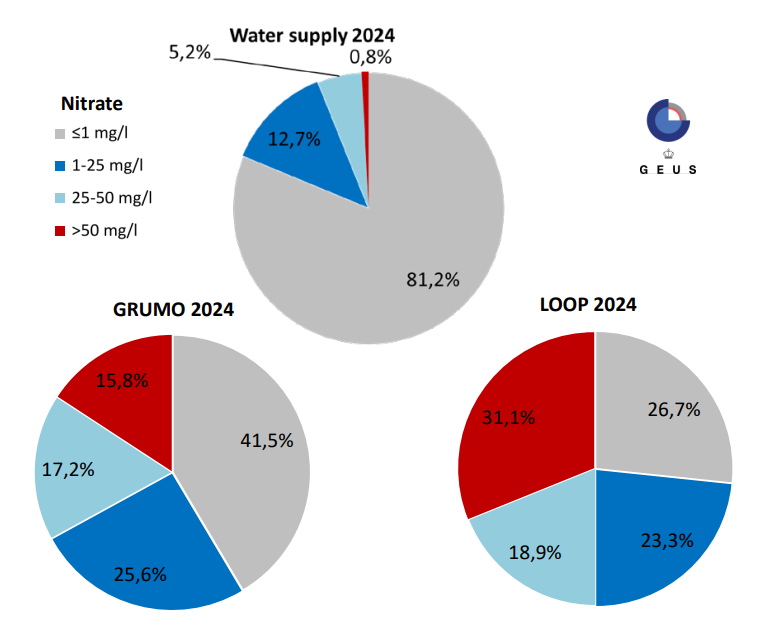
\includegraphics[width = .8\textwidth]{figures/nitrateCakes.png}
    \captionof{figure}{ \footnotesize From GEUS' groundwater report
    2025~\cite{laerke_thorling_groundwater_2025}.}
\end{frame}

\begin{frame}{Nitrate pollution in Denmark}
    \center 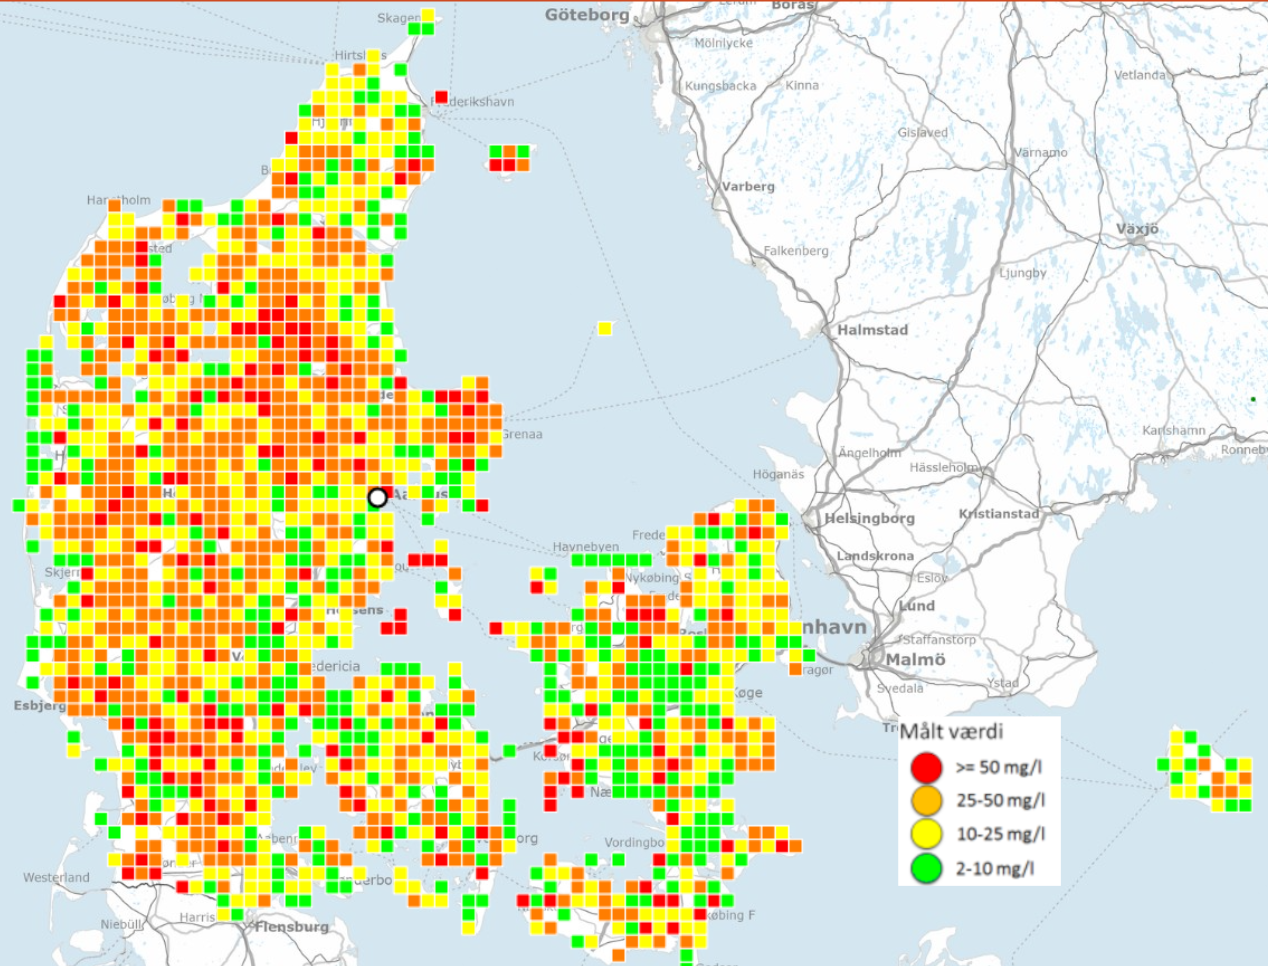
\includegraphics[width = .8\textwidth]{figures/nitrateMap.png}
    \captionof*{figure}{
    \tiny\url{https://www.geus.dk/produkter-ydelser-og-faciliteter/data-og-kort/grundvandskort-og-data}}
\end{frame}

\begin{frame}
        \begin{center}
            
\includegraphics[width=\textwidth]{figures/wrestlingPFAS.png}
        \end{center}

    \Huge\bf
    \textcolor{msred}{
    PFAS - the Immortal}
\end{frame}

\begin{frame}
    \center 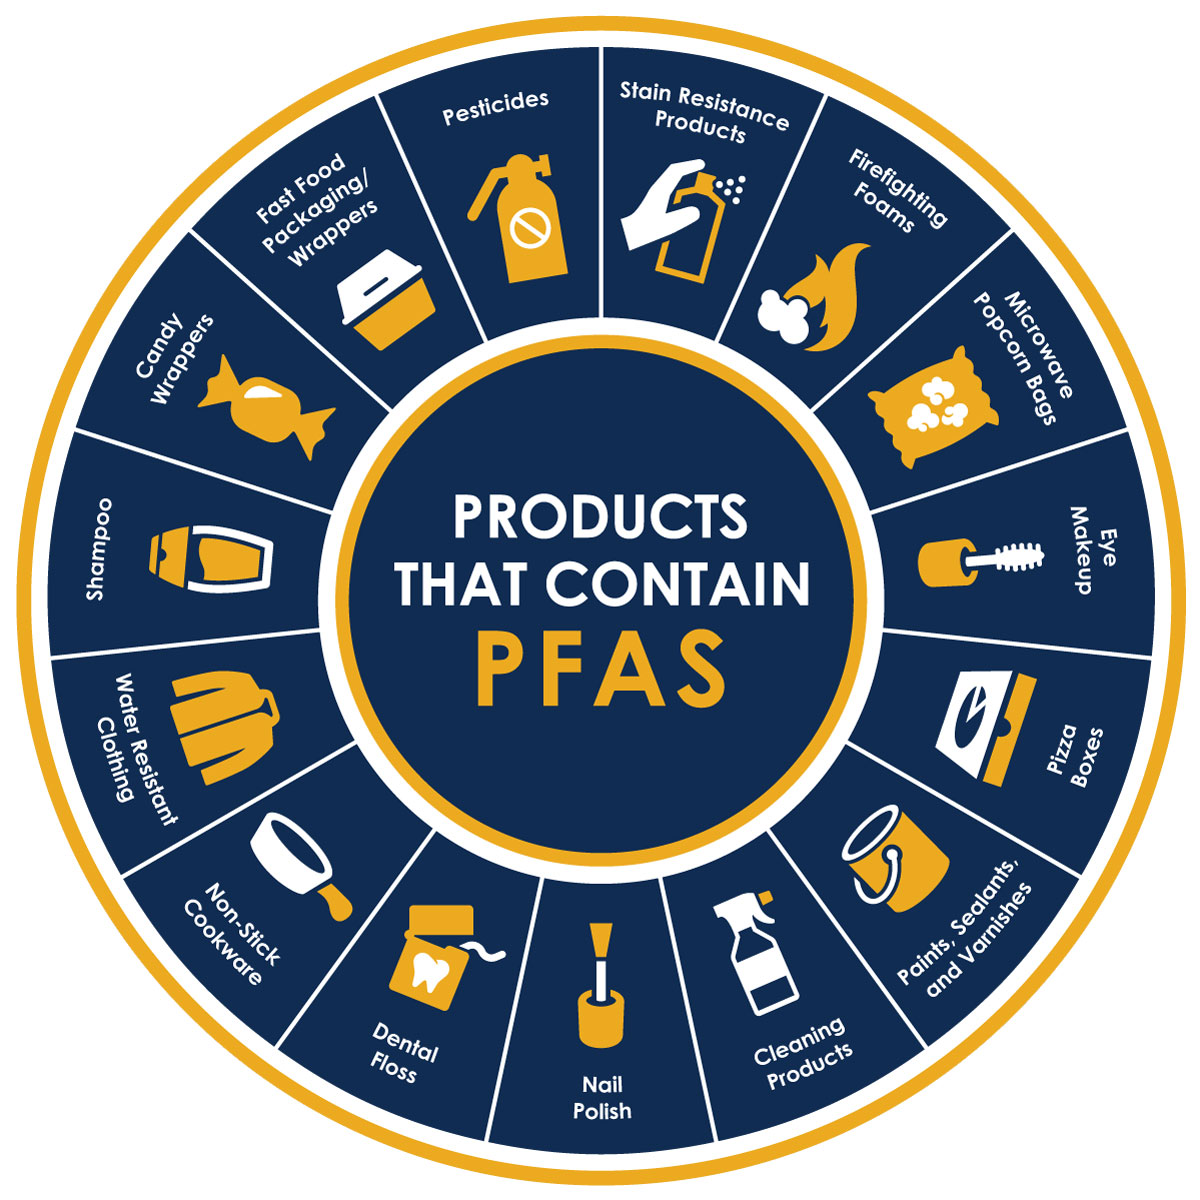
\includegraphics[width = .8\textwidth]{figures/RPU Products Containing PFAS.jpeg}
    \captionof*{figure}{\footnotesize Infographic by the Californian government}
\end{frame}

\begin{frame}
\begin{minipage}{\textwidth}
    \center 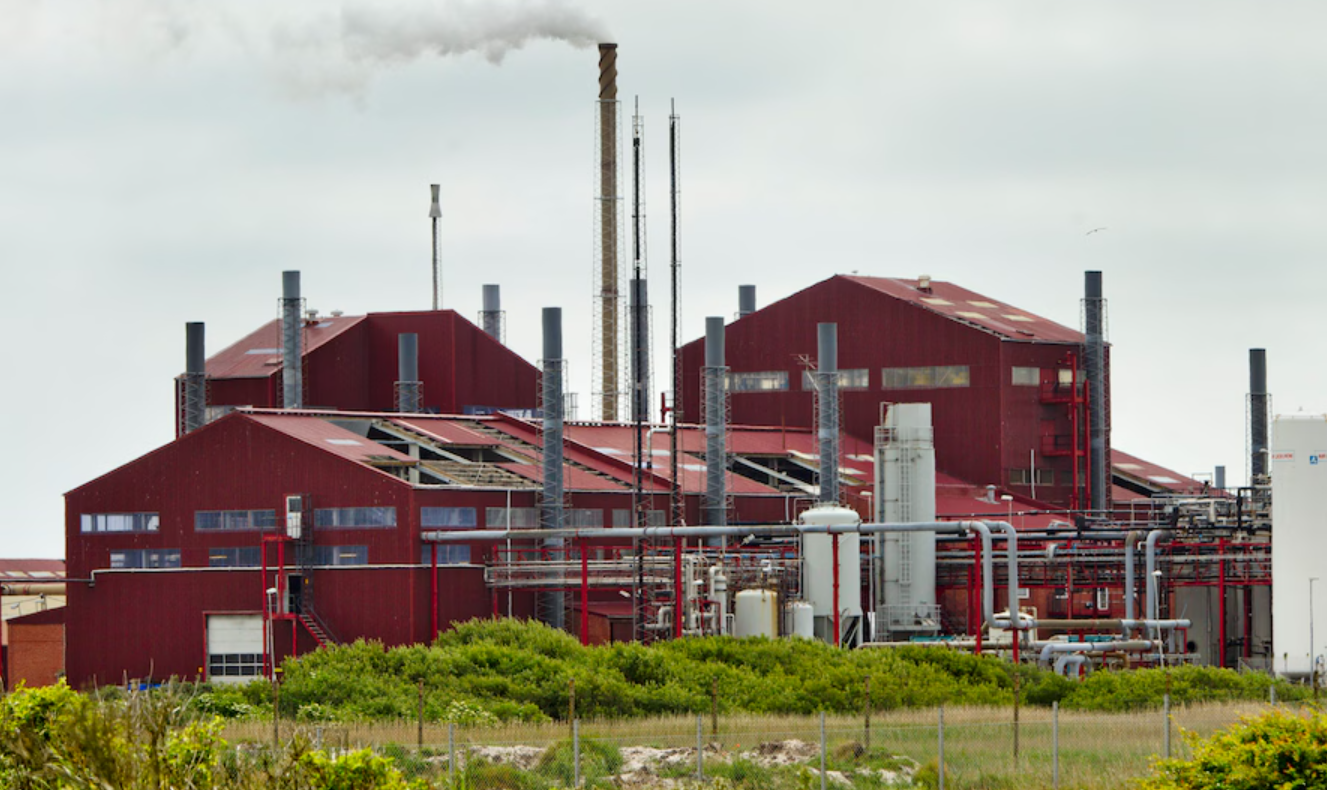
\includegraphics[width = .8\textwidth]{figures/cheminova.png}
    \end{minipage}

    \begin{minipage}{\textwidth}
    \center 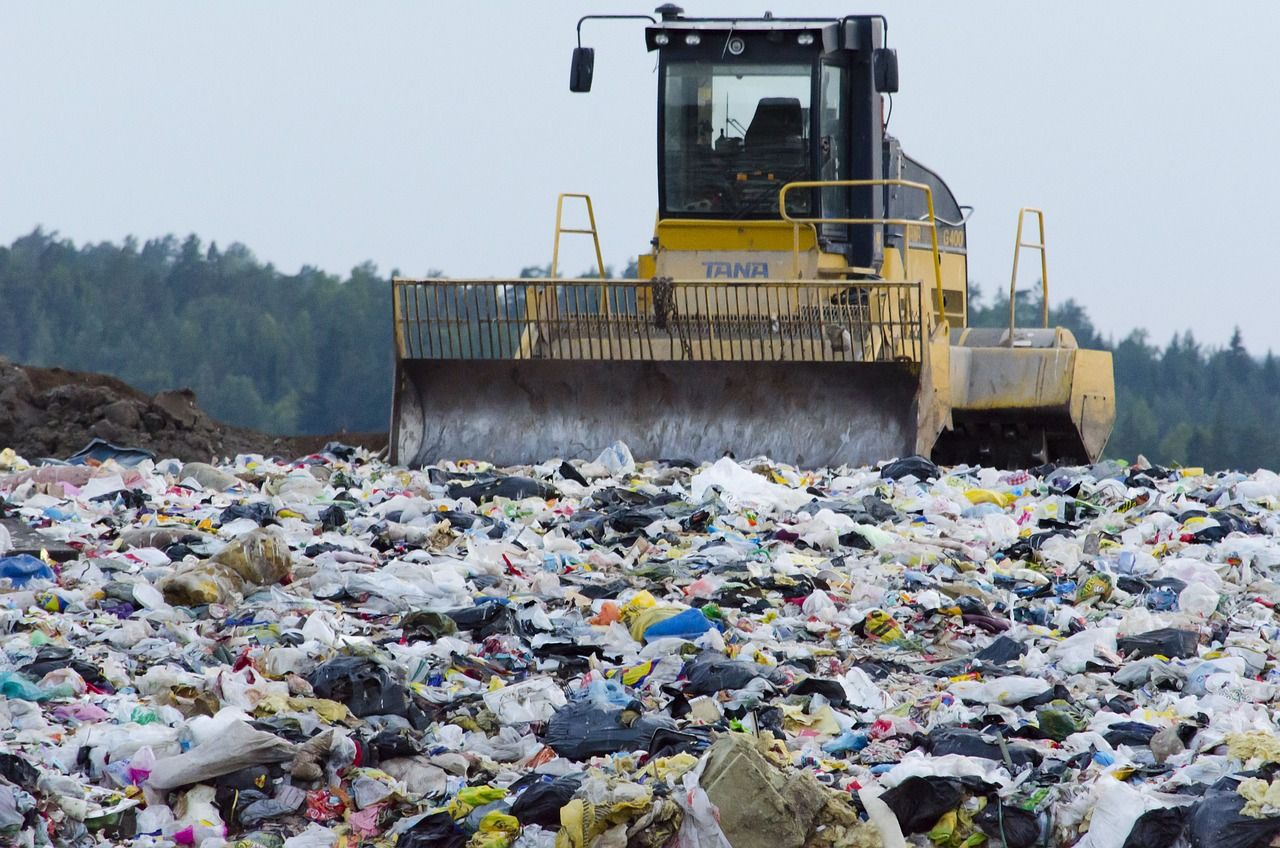
\includegraphics[width = .8\textwidth]{figures/landfill.jpg}
    \end{minipage}
\end{frame}


\begin{frame}{Where do they live?}
    \textbf{Where DON'T they live!?}
    PFAS are found in water, air, fish, and soil..\pause

    Also, in blood of people, animals, in food
    products\footnote{\url{https://www.epa.gov/pfas/pfas-explained}}

\end{frame}

\begin{frame}{PFAS measurements in groundwater wells}
    \centering
    \center 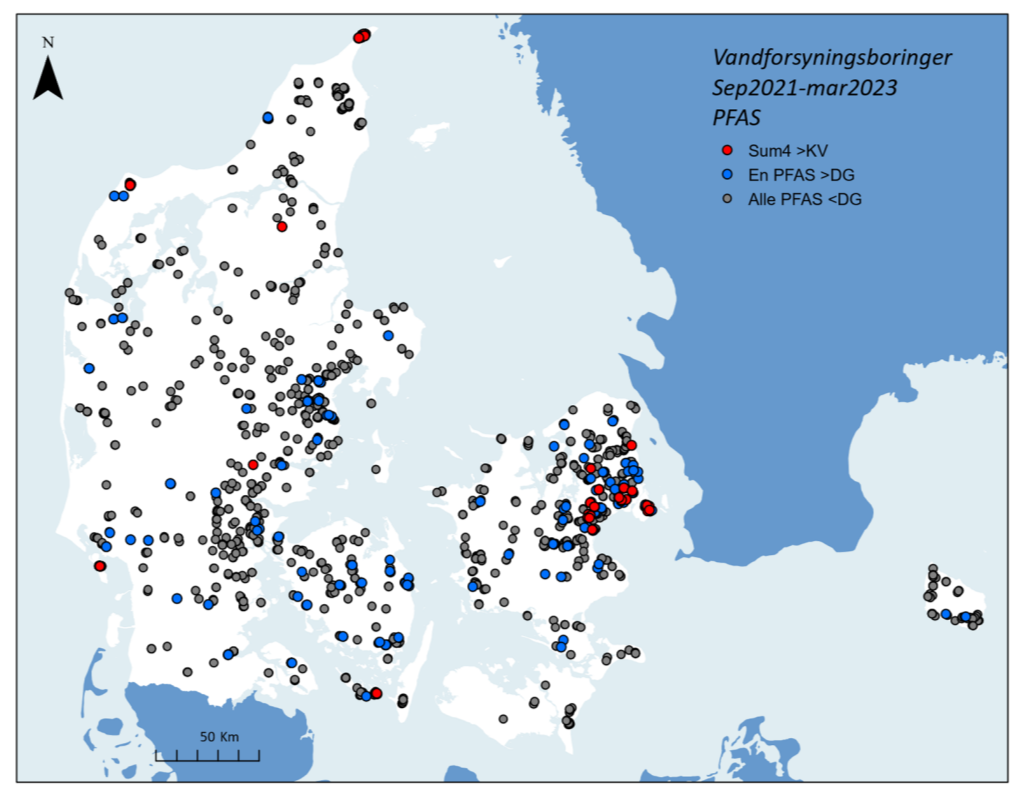
\includegraphics[width = .75\textwidth]{figures/pfasMeas.png}

    \captionof*{figure}{\footnotesize\emph{Red:} PFAS chemicals above limit.
        \emph{Blue:} Measured PFAS chemicals. \emph{Grey:} None
    detected~\cite{anders_r_johnsen_laerke_thorling__christian_n_albers_pfas-stoffer_2023}.}

\end{frame}

\begin{frame}{PFAS measurements in groundwater wells}
    \centering
    \center 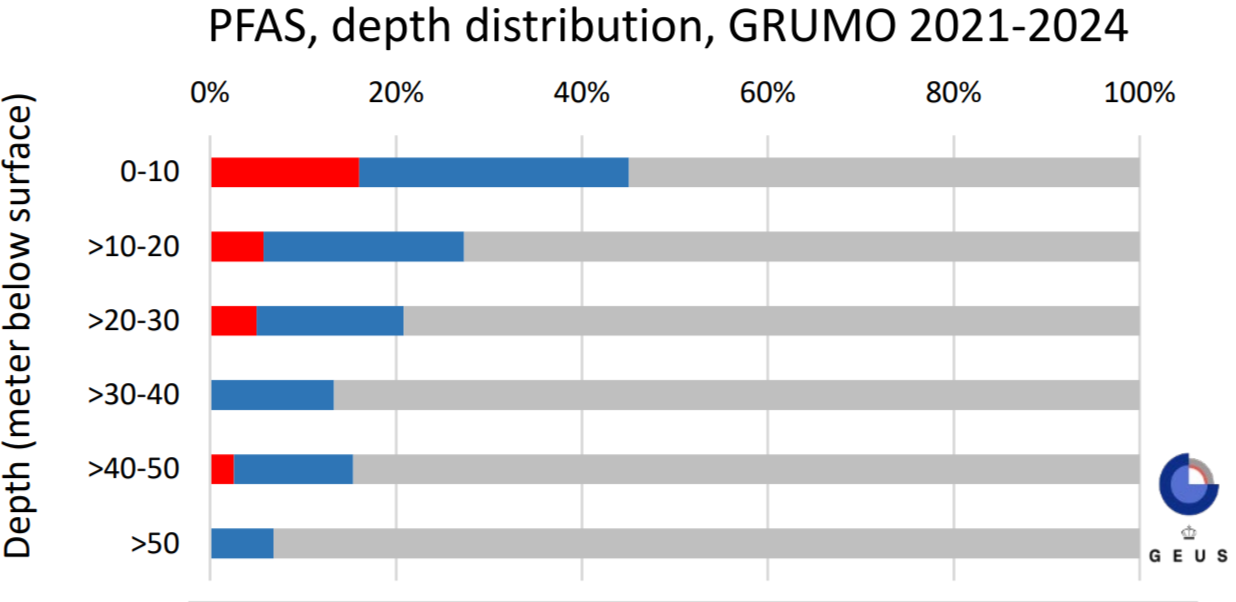
\includegraphics[width = .75\textwidth]{figures/pfasdepth.png}

    \captionof*{figure}{\footnotesize\emph{Red:} PFAS chemicals above limit.
        \emph{Blue:} Measured PFAS chemicals. \emph{Grey:} None
    detected~\cite{laerke_thorling_groundwater_2025}.}

    PFAS does not simply break down. They're the eternity chemicals.
\end{frame}



\begin{frame}{Big promises}
    \begin{itemize}
        \item Protect 160 thousand hectar against pesti- and herbicides.
        \item 30 \% of Denmark will be protected.
        \item Reduce environmental impact of especially pig farms.
    \end{itemize}
    
\end{frame}



\begin{frame}{Big promises}
    Already theres been strong push back by the Landbrug \& Fødevarer~\cite{noauthor_gron_2026}
    \pause
    \vspace{1em}

    Environmental organisations like DN are cautiously optimistic~\cite{noauthor_eksisterer_nodate}
    \pause
    \vspace{1em}

    The report is quite unspecific about e.g. PFAS and reduction of stock animals.
\end{frame}



% Part 2
% -----------------------------------------------------------------------------
\begin{frame}{ToC}
    \Large{Part Two:}
    \begin{itemize}
        \item Case studies in the global south
        \item How are we as Europeans involved?
        \item How is climate change changing the picture?
    \end{itemize}
\end{frame}


\appendix
\begin{frame}[allowframebreaks]
    \frametitle{References}
    \bibliographystyle{ieeetr}
    \bibliography{./refs.bib}
\end{frame}

\end{document}
